\subsection{Architectural Views}

\subsubsection{Logical View} % which is the object model of the design, end-user functionality (Class diagrams)
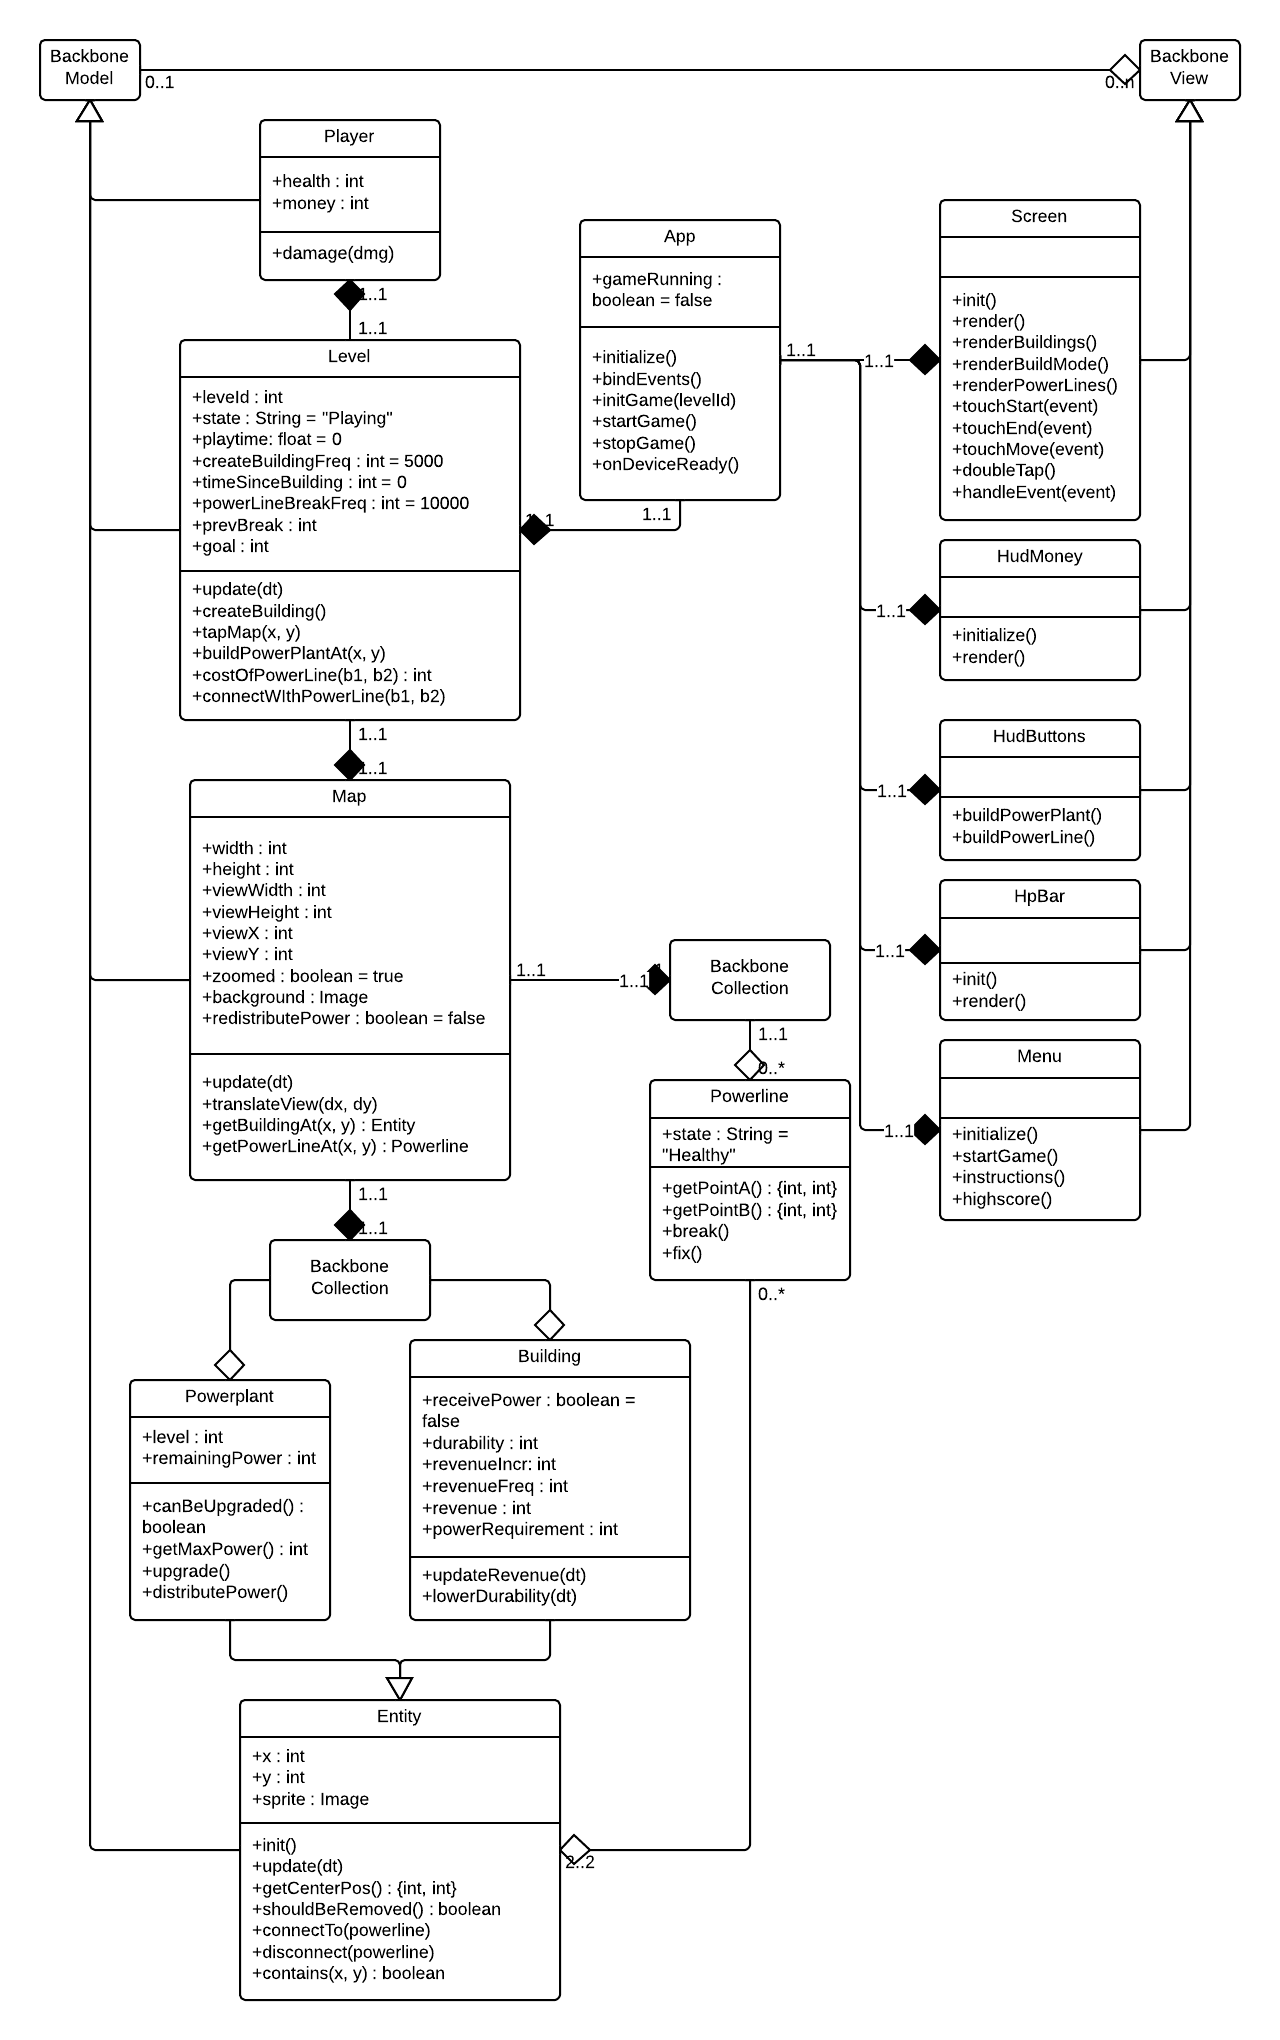
\includegraphics{/pictures/class_diagram}

-->> The screen class will probably become connected to more classes as the GUI is planned. <<--

\subsubsection{Process View} % captures the concurrency and synchronization aspects of the design, itegrators, performance, scalability. Takes into account some non-functional requirements, like performance and reliability.

\subsubsection{Physical View} % describes the mappings of the software onto the hardware, and reflects its distributed aspect, system engineers, topology, communications
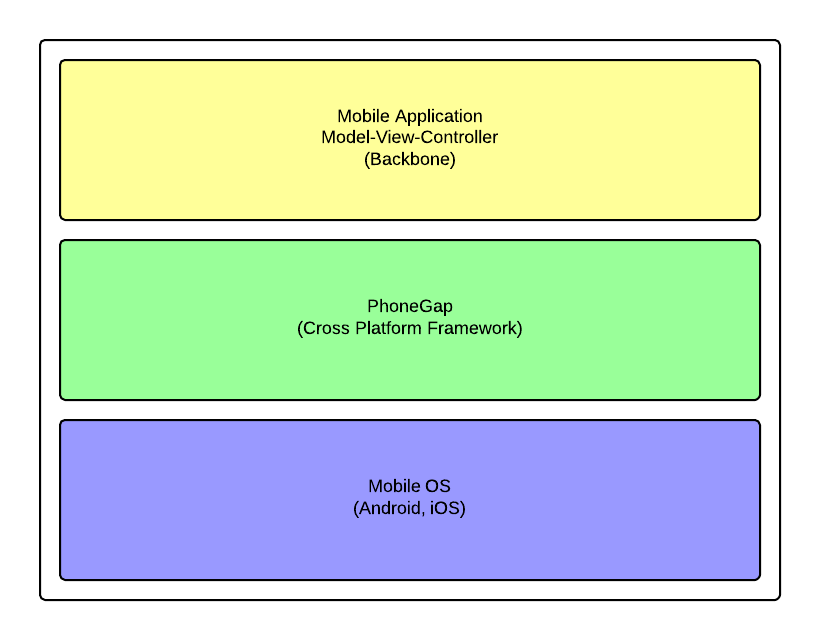
\includegraphics{/pictures/physical_view}

The physical architecture of our product is seperated into 3 layers. Platform specific issues are handled using PhoneGap as a cross platform framework between the application and the mobile OS.

{\bf Layer 1 - Native platform}
The first layer is the native operative system that runs on the device. This layer handles touchscreen functionality, rendering to screen, data input/output and other platform specific features.

{\bf Layer 2 - Cross platform framework}
The cross platform framework is called PhoneGap. The purpose of this layer is to allow the development team to write portable code that can run on both Android and iOS, without having to develop for both Android and iOS separately in 2 different programming languages. PhoneGap uses browser functionality on each platform to run HTML5, CSS and JavaScript code and provides access to platform functionality like camera and touchscreen.

{\bf Layer 3 - Mobile Application}
The third layer is where the game is implemented using the MVC pattern. 


\subsubsection{Development View} % describes the static organization of the software in its development environment, programmers, software management

\subsubsection{Scenarios} % Bla bla bla, and the illustrated by a few selected use cases, or scenarios which becomes a fifth view
